% !TeX root = ../../Thesis.tex
\section{Modelling the Physical Problem}
This section describes the evaporation of superheated fluids. The existing literature
documenting the phenomenological process is reviewed, along with the modelling
of nucleation, bubble growth, and the various methods to model flash evaporation.
Additionally,  the mathematical framework and governing equations used to model the two-phase flow problems are introduced.
The rationale behind averaging techniques for multiphase flow modelling is explained and the 
macroscopic formulations of the one-fluid and two-fluid models are presented. 
Multiphase turbulence is addressed and the two subproblems and their parameters(?) 
are defined. 


\subsection{Evaporation}
Evaporation processes are characterised based on whether they occur at saturation
temperatures or not. Evaporation at saturation temperatures, known as vaporisation, is a much
faster process in comparison to evaporation at normal temperatures. 
Here, the metastability of liquids becomes relevant and the inception of vaporisation
is governed by how far a liquid can enter the metastable zone. A liquid that is heated 
above its equilibrium saturation temperature without undergoing phase change 
is termed as being metastable. The degree of superheat is 
\begin{equation}
  \Delta T \;=\; T - T_{\ind{sat}}\,,
\end{equation}
where \(T\) is the temperature of the bulk liquid and \(T_{\ind{sat}}\) is the 
saturation temperature at the system pressure. The intensity of vaporisation
is strongly dependent on the degree of superheat.~\cite{wickertSimulation, pinhasiModelingFlashingTwoPhase2005}


In cases where vaporisation occurs along a heated wall, most CFD models distribute the energy 
transfer by separating the wall heat flux into two components: 
latent heat absorption associated with bubble vaporisation and 
sensible heat transferred to the liquid through conduction, 
convection, and quenching processes. The partitioning depends on 
the area fractions covered by liquid and vapour phases.
Empirical results or models of subprocesses have 
established correlations between the heat flux and wall superheat.~\cite{gilmanDevelopmentGeneralPurpose2014,ghiaasiaanTwoPhaseFlowBoiling2007}


\subsubsection{Vaporisation: Phenomenological and Literature Review}
Boiling processes take place due to consistent heat transfer to the system and takes place on the heated surface. 
Additionally, boiling of pure liquids is an isothermal process that is 
driven by the difference between the hot surface and the liquid. 
Flash evaporation is the intense vaporisation triggered through depressurisation 
of superheated fluids below the saturation pressure.
This process induces a violent and transient heat
and mass transfer, resulting in the explosive formation and growth
of vapour bubbles throughout the liquid volume. The phenomenon is significant 
in desalination on ships, nuclear reactor safety, and venting of cryogenic
propellant tanks, and the harvesting of low-temperature geothermal energy.~\cite{sauryExperimentalStudyFlash2002, wuExperimentalStudyFlash2019, liaoReviewNumericalModelling2021, mutairExperimentalInvestigationCharacteristics2010, vahajiEfficiencyTwophaseNozzle2014}


Early experiments that systematically studied flash evaporation in liquid pools and sprays in superheated 
water jets and early empirical correlations to determine the amount of generated 
vapour were established~\cite{miyatakeExperimentalStudySpray1981, miyatakeEffectLiquidTemperature1981, gopalakrishnaExperimentalStudyFlash1987, petersonInvestigationsLiquidflashingEvaporation1984}.
For flash evaporation in static pools, the amount of liquid height increased the duration 
of the phenomenon and the rate of depressurisation increases the intensity.
The final evaporated mass also increases proportional to the amount of superheat.
While greater thermal inertia at larger depths slows the flashing process, the amount of total 
mass evaporated does not increase proportionally.~\cite{sauryFlashEvaporationWater2005,sauryExperimentalStudyFlash2002}
It has been observed during flashing, that a liquid-vapour interface is generated 
on the free surface which then progresses into the superheated liquid~\cite{mansourReviewFlashEvaporation2019, HahneBarthau2000, reinkeExplosiveVaporizationSuperheated2001}.
High-speed imaging and temperature measurements consistently show that
flash evaporation proceeds through three distinct stages: bubble generation,
boiling growth, and a boiling reduction stage~\cite{wuExperimentalStudyFlash2019}.
%For the final evaporated mass, under moderate superheat conditions \(\Delta T \leq 35\,\munit{K}\),
%a strong linear scaling is observed~\cite{liaoFlashingEvaporationDifferent2013,liaoReviewNumericalModelling2021}.


Parameters like the non-equilibrium fraction (NEF) and non-equilibrium temperature difference (NETD) have been proposed to 
quantify the flash evaporation phenomenon. Correlations between the evaporated mass and the dependency on temperature 
have been obtained by fitting curves to experimental data under various operating conditions. However,
the experimental study of the physics remains a challenge due to the inadequacy of measurement techniques that
can measure local flow phenomenon accurately. Numerical simulations generally also use the empirical assumptions 
and relations from specific experiments, making the extension to a general case difficult.~\cite{haoMathematicalStudyBubble2019}


\begin{figure}[ht]
\centering
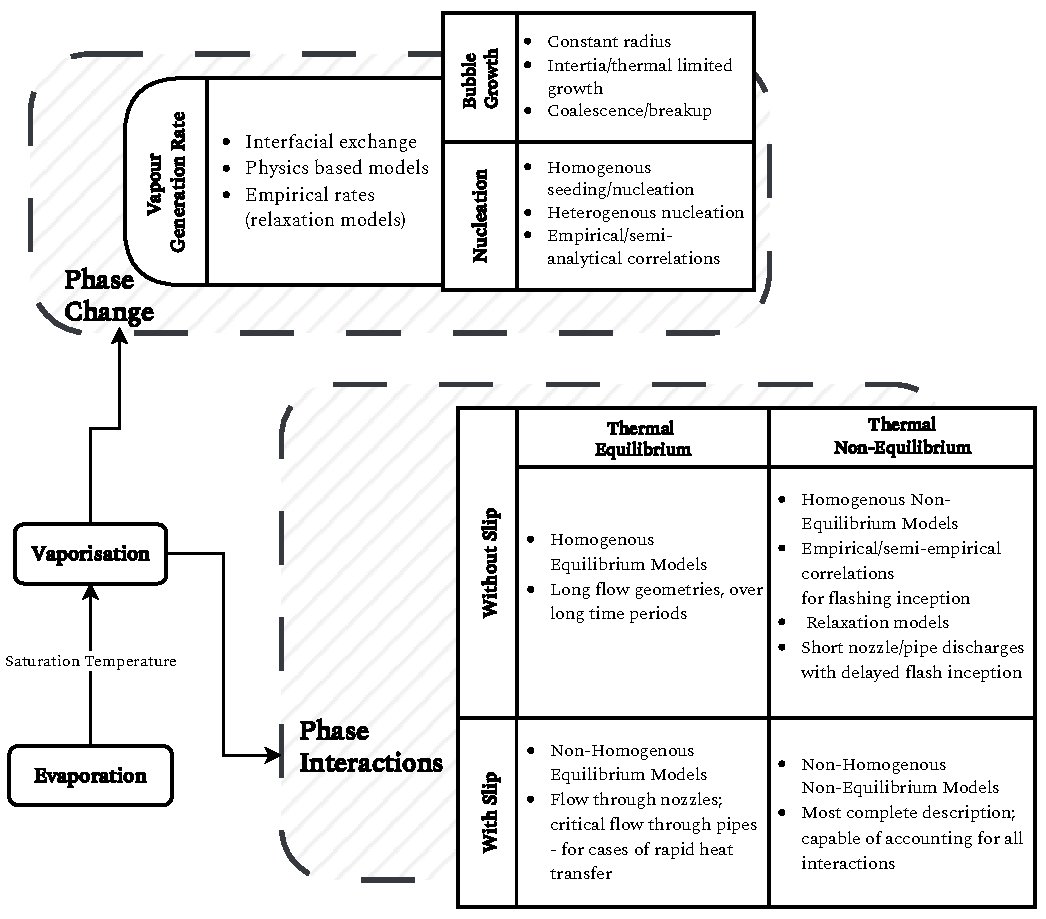
\includegraphics[width=1.\linewidth]{Chapters/Chap1/figs/flowchart_flashing2}
\caption{Categorisation of flash evaporation models}
%\label{\fig{rt_conv_3000}} % \fig used here
\end{figure}
The approaches to modelling flash evaporation can be differentiated by:
\begin{itemize}
  \item the level of complexity captured in the phase change modelling process, and
  \item how the interaction between the phases is modelled.
\end{itemize}
Interaction between the phases can be distinguished primarily through the consideration of thermal non-equilibrium or
relative (slip) velocity between the phases~\cite{liaoComputationalModellingFlash2017}. 
\begin{itemize}
  \item \textbf{Homogenous Equilibrium Models (HEM)} assume thermal equilibrium and no slip velocity between the phases. 
  Similar to the one-fluid formulation described in \sect{sec:one-fluid} where the thermodynamic properties are interpolated from tables or constitutive relations.
  Sometimes applicable for flows in long pipes where the phases have enough time to achieve equilibrium, HEM tends to underpredict flow rates and
  is incapable of predicting early time non-equilibrium thermal effects and later time momentum non-equilibrium effects between the phases.
  \item \textbf{Non-Homogenous Equilibrium Models (NHEM)} treat the system as a mixture but account for slip velocities. With gas volume fractions over \(0.3\),
  the relative motion between the phases become significant. However, correlations for the interphase relative motion tend to over-predict the 
  flow rates in comparison to the two-fluid model, described in \sect{sec:two-fluid}, that assumes thermal and velocity non-equilibrium.
  %Determines the slip ratio parametrically by analysis for which slip ratio the mass flow rate is maximum
  \item \textbf{Homogenous Non-Equilibrium Models (HNEM)} assume thermal non-equilibrium but do not account for the relative motion between the liquid and vapour phases.
  While assuming thermal equilibrium underpredicts vapour generation in short geometries, limited understanding of the non-equilibrium physical phenomena such as nucleation 
  and interphase transfers can lead to equally unphysical results while accounting non-equilibrium. HNEMs are primarily boiling delay models based on physical or empirical 
  observations and relaxation models. The boiling models try to emulate the nucleation process as a quasi-step function or trigger flashing inception at a certain
  superheat threshold. Mixture models need accurate modelling of the vapour generation, interphase momentum transfer, and nucleation rate. Relaxation models
  solve a rate equation along with a homogenous equilibrium model - the rate equation, based on empirical relaxation times, 'relaxes' the non-equilibrium mixture to the 
  equilibrium state.
  \item \textbf{Non-Homogenous Non-Equilibrium Models (NHNEM)} such as the drift-flux and two-fluid models are the most general formulations. Although the drift-flux model can
  be used to model the slip between phases based on other flow field variables, it can't accurately capture non-equilibrium effects. The two-fluid model provides the most 
  general formulation to model flash evaporation, however all interactions and non-equilibrium exchanges must be accurately modelled. The drift-flux model provides a good compromise between
  the modelling complexity and computational efficiency between the HNEM and the two-fluid formulations.
\end{itemize}
\cite{dangleComputationalFluidDynamics2018,liaoComputationalModellingFlash2017,liaoReviewNumericalModelling2021}


The phase change modelling process can be extended to account for the various sub-processes observed in flash evaporation phenomena:
\begin{itemize}
    \item nucleation and number density of nucleation sites,
    \item bubble growth, diameter at time of detachment, frequency of detachment,
    \item and interactions between the bubbles.
\end{itemize}\cite{dangleComputationalFluidDynamics2018}
Phase change can also be modelled simply by assuming a constant bubble number density and diameter disregarding bubble 
growth or nucleation rates. Artificial coefficients based on empirical relations or assumptions can be used to accommodate the non-equilibrium effects.
Mono-disperse assumptions for bubble sizes, however, tend to have inherent limitations in reproducing accurate bubble dynamics.~\cite{liaoNumericalAnalysisFlashing2019}


Nucleation affects the number and distribution of bubbles in the fluid. Walls - particularly so in case they're heated - are more susceptible 
to be nucleation sites for bubble growth
as the activation energy is much lower. This nucleation can be modelled through the domain as homogenous or heterogeneous - where nucleation sites are modelled using a 
presumed PDF function or be determined by empirical correlations.~\cite{liaoComputationalModellingFlash2017}


After a stable bubble nucleus has been formed, the growth of the bubble becomes pertinent in the evaluation
of the diameter at departure and the interphase energy and mass transfer. In the case of an ideal
spherical bubble undergoing expansion in a uniformly superheated liquid, the rate of growth
is determined by the surface tension, liquid inertia, and the difference in pressures inside
and outside the bubble. Surface tension dominates and restricts the initial bubble growth.
This initial rapid expansion of the bubble results in the formation of a thin liquid layer separating
the vapour from the wall surface. This microlayer can be a significant contributor to the 
bubble growth and heat transfer process.
As bubble radius increases, the liquid layer surrounding the bubble 
cools due to evaporation, resulting in a decrease in vapour pressure. 
The bubble growth dynamics are initially governed by thermal diffusion 
and inertia. Over time, inertial effects become less important as 
the bubble expands more slowly. Further growth is determined 
primarily by interphase energy exchange.~\cite{sherFlashboilingAtomization2008}


\subsubsection{Effects of low pressure and gravity conditions}
The absence of significant gravitational forces alters the dynamics of vaporisation - affecting natural convection, buoyancy
driven phenomenon, and bubble dynamics. Under terrestrial gravity, convection currents develop under thermal
gradients, thus bringing cooler liquid to the heated surface as the vapour bubble rises due
to buoyancy. This density driven natural convection is affected in low gravity conditions, maintaining
the thermal gradient. Bulk fluid movement is affected and heat and mass transfer processes shift
from being convection dominated to being diffusion dominated.~\cite{cochranEffectsFluidProperties, leeExperimentalComputationalInvestigation2022}


In nucleate boiling under low gravity conditions, vapour bubbles tend to remain near the heat source, growing
significantly larger and coalescing with smaller bubbles. Prolonged bubble presence on the
surface results in drying out of the surface and unsteady rise in surface temperatures during nucleate boiling.\cite{qiuSingleBubbleDynamicsPool2002}~\COMMENT{Mention some numbers}
In conditions where the dominance of surface tension forces becomes more pronounced,
the surface tension gradients can induce fluid circulation. This is known as Marangoni
convection and is observed to affect bubble growth and heat transfer.~\cite{xuNumericalStudyMarangoni2014}
Recent experiments studying stationary volatile drop evaporation in microgravity
report a \(56\%\) reduction in evaporation rate as compared to normal gravity conditions~\cite{kumarSessileVolatileDrop2020}


Reduced system pressure impacts the overall intensity of heat transfer. The onset of nucleate boiling also
requires higher superheat values in low pressure conditions.
Decrease in pressure leads to a lower number of active nucleation sites and increases
microlayer thickness found at the bubble-wall interface. A decreased amount of
bulk nucleation is reported along with the increased relevance of bubble growth. 
An over-prediction is vapour mass generation is reported since large bubbles decrease
the interfacial area density.~\cite{serdyukovInfluencePressureLocal2023, zhangExperimentalTheoreticalStudy2002,liaoFlashingEvaporationDifferent2013}


\subsection{The Physics and Thermodynamics of Flash Evaporation}
%Although comparable to cavitation, where phase change and bubble nucleation are 
% also observed due to a pressure drop, flashing is differentiated 
% due to the sustenance of the bubbles formed and the higher temperatures 
% observed during flashing~\cite{pinhasiModelingFlashingTwoPhase2005}.
Flash evaporation is triggered when the superheat limit is reached.
The limit of superheat can be the thermodynamic or the kinetic limit based
on thermodynamical and kinetic theory considerations respectively. 
The absolute thermodynamical limit, also known as the spinodal limit, is never
practically attained. Vaporisation is always triggered much before the spinodal limit due to 
internal impurities, density fluctuations, wall nucleation, or  the presence of 
pre-existing nuclei.~\cite{pinhasiModelingFlashingTwoPhase2005,liaoComputationalModellingFlash2017}


The maximum 
degree of superheat or the pressure undershoot determines the behaviour of the
subsequent boiling. The pressure undershoot is defined as the difference between
the minimum pressure after depressurisation and the saturation pressure corresponding
to the initial temperature.

\begin{figure}[h]
  \centering
  \begin{subfigure}[t]{0.5\textwidth}
    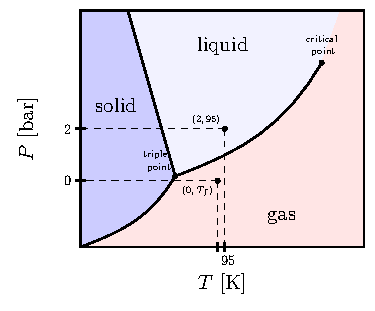
\includegraphics[width=\linewidth]{./Chapters/Chap1/figs/water_phase_diag}
    \caption{Phase diagram of water with approximately marked initial and final experimental conditions.}
  \end{subfigure}
  \hfill
  \begin{subfigure}[t]{0.48\textwidth}
    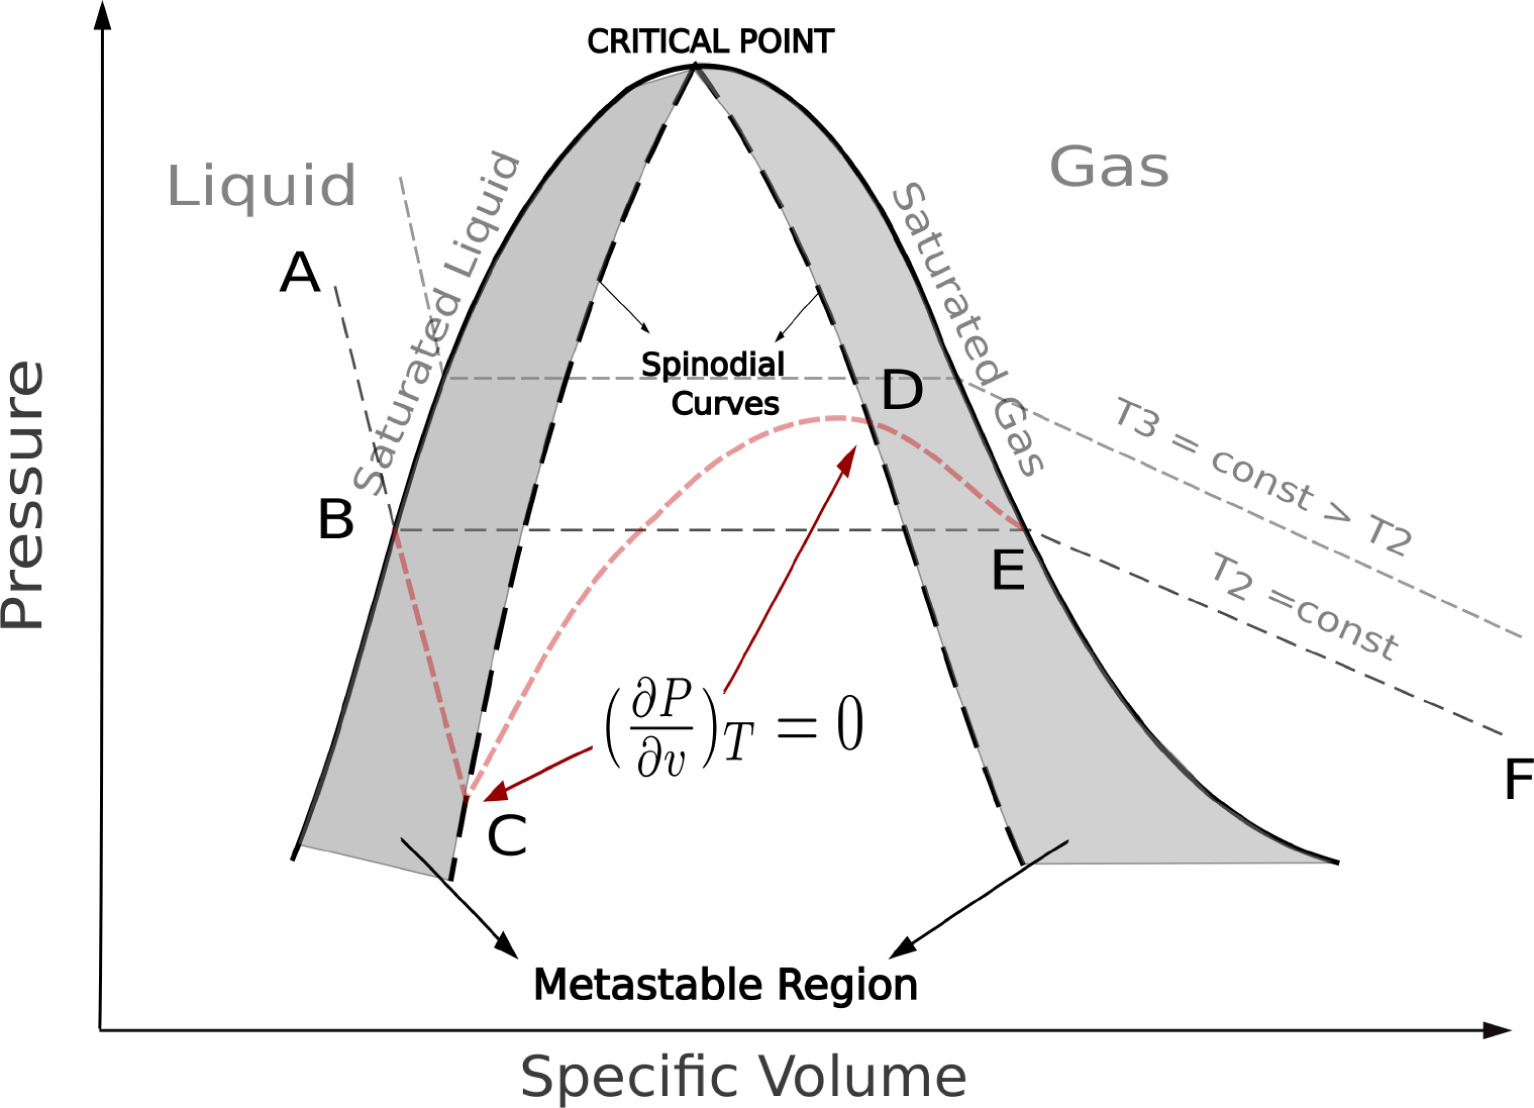
\includegraphics[width=\linewidth]{./Chapters/Chap1/figs/spinodal.jpg}
    \caption{Spinodal lines and metastable regions for a liquid on a P-v diagram.}
  \end{subfigure}
  \caption{Thermodynamic stability of water}
\end{figure}
Phase transition starts with a random 
aggregation of molecules to form a 'nucleus' with the properties of the new phase. 
Nucleation modelling allows the estimation of the size of the unstable bubble embryos 
at the moment of flashing inception. Homogenous nucleation establishes the conditions for a bubble embryo to be in equilibrium with 
the surrounding superheated liquid. Energetically, a
curved surface is characterised by its free surface energy which for a curved liquid-vapour
interface is essentially the surface tension, \(\sigma\). 
The change in Gibbs free energy \(\Delta G\) associated with the formation of a bubble of radius
\(R_{\ind{i}}\) with volume \(\frac{4}{3} \pi R_{\ind{i}}^{3}\) in a superheated liquid, as described in~\eq{eq:delta-gibbs},
can be given using the specific Gibbs free energies \(\hat{g}_{\ind{i}}\), 
the number of moles \(\hat{N}_{\ind{i}}\), the pressure \(p_{\ind{i}}\), where \(i\,=\,\{\ind{l},\ind{v}\}\)
for the liquid and vapour phase respectively.
\begin{equation}\label{eq:delta-gibbs}
  \Delta G \;=\; \hat{N}_{\ind{v}}(\hat{g}_{\ind{v}} - \hat{g}_{\ind{l}}) 
  + 4\pi R_{\ind{i}}^{2} \sigma 
  - \frac{4}{3} \pi R_{\ind{i}}^{3}(p_{\ind{v}} - p_{\ind{l}}),
\end{equation}
For a bubble with the critical radius \(R_{\ind{e}}\) at thermodynamic and mechanical equilibrium 
with the superheated fluid, the chemical potentials of the two phases must be equal
and the momentum jump equation - the Young-Laplace equation must be satisfied.
\begin{subequations}
  \begin{align}
    \hat{g}_{\ind{v}} & = \hat{g}_{\ind{l}},\\
    p_{\ind{v}} - p_{\ind{l}} & = \frac{2\sigma}{R_{\ind{i}}},
  \end{align}
\end{subequations}
{}~\eq{eq:delta-gibbs} at equilibrium conditions between the bubble and the liquid, 
thus reduces to 
\begin{equation}
  \Delta G_{\ind{e}} = 4\pi R_{\ind{e}}^{2} \sigma - \frac{4}{3} \pi R_{\ind{e}}^{3}\frac{2\sigma}{R_{\ind{e}}} = \frac{4}{3} \pi R_{\ind{e}}^{2} \sigma,
\end{equation}
The equilibrium is unstable as seen in~\fig{FIG}, and the loss of one molecule from
the bubble embryo will lead to bubble collapse. Conversely, a bubble embryo with radius greater than
\(R_{\ind{e}}\) is expected to spontaneously grow - resulting in homogenous nucleation of the vapour phase in the system.
 %%%%%%%%%%%%%%%%%%%%%%%%%%%%%%%%%%%%%%%%%%%%%%%%%%%%%%%%%%%%




\subsection{Modelling Multiphase Flows}
The computational tribulations of directly solving local instantaneous governing equations throughout 
 the entire domain necessitates dimensional reduction through macroscopic formulations. 
 For two-phase flows (used interchangeably with multiphase flows), these formulations rely 
 on averaging local flow field fluctuations while preserving continuum mechanics principles. 

In the following, we use the subscript \(i \in \{l, v\}\)~\COMMENT{(and \(j\) such that if \(i = l\), \(j = v\))}
 to denote variables associate with the 
 liquid (\ind{l}) and vapour (\ind{v}) phase respectively. Figure~\fig{FIG} % \fig used here
displays a region \(\Omega\) where two phases \ind{l}, \ind{v} occupy
 regions \(\Omega_{\ind{l}}(t)\) and \(\Omega_{\ind{v}}(t)\) such that \(\Omega = \Omega_{\ind{l}}(t) \cup \Omega_{\ind{v}}(t)\) is constant in time.     
 The boundaries of the domains - \(\partial \Omega_{\ind{l}}\), \(\partial \Omega_{\ind{v}}\), and \(\partial \Omega\) - together define the interface that separates the two phases as
\begin{equation}
  \mathcal{S}(t) \;=\;\Bigl(\partial\Omega_{\ind{l}} \cap \partial\Omega_{\ind{v}}\Bigr)\setminus\partial\Omega\,.
  \label{eq:interface}
\end{equation}~\COMMENT{Equation seems a bit pretentious or? also idk if is a good choice for notation}
Eulerian averaging is related to the Eulerian description of the flow - the local instantaneous
variables are averaged with the time and space variables being kept constant.
Volume averaging admits a general 
representative volume element \(V\) bounded by \(\partial V\), and 
time averaging uses a time interval at
every spatial reference point \((\vect{x}, t)\) in the region.
The averaging volume \(V\) is partitioned into \(\textstyle \sum V_{\ind{i}}\) with the volume fraction for phase \(i\) being
\begin{equation}
  \alpha_{\ind{i}}(\vect{x},t) \;=\; \frac{V_{\ind{i}}}{V}\,,\qquad
  \alpha_{\ind{l}} + \alpha_{\ind{v}} = 1\,.
  \label{eq:volfrac}
\end{equation}

All averaging procedures generally utilise a phase indicator function that 
 marks the presence of the phase in the averaging domain. Denoted as \(\gamma_{\ind{i}}\), 
 the phase indicator function can be used to define the average of the general scalar or vector quantity \(\psi\) over the averaging 
 volume \(V\),
\begin{equation}
  \overline{\psi_{\ind{i}}}^V
  \;=\;
  \frac{1}{V}\integ{V}{} \gamma_{\ind{i}}\,\psi_{\ind{i}}(\vect{x},t)\,\diff{V}\,,
  \label{eq:volavg}
\end{equation}\cite{ishiiThermoFluidDynamicsTwoPhase2011, ishiiThermoFluidDynamicsTwoPhase2011}
and the phase-intrinsic average then is
\begin{equation}
  \overline{\psi_{\ind{i}}}^{\ind{i}} \;=\;\frac{1}{V_{\ind{i}}}\integ{V_{\ind{i}}}{}\psi(\vect{x},t)\,\diff{V}
  \;=\;
  \frac{\overline{\psi_{\ind{i}}}^V}{\alpha_{\ind{i}}}\,.
  \label{eq:intravg}
\end{equation}

% Example: temperature in Kelvin (unit)
%The temperature \(T\) at which phase change occurs is typically about \(T_{\ind{sat}} = 373\,\munit{K}\).
\begin{figure}[h]
\centering
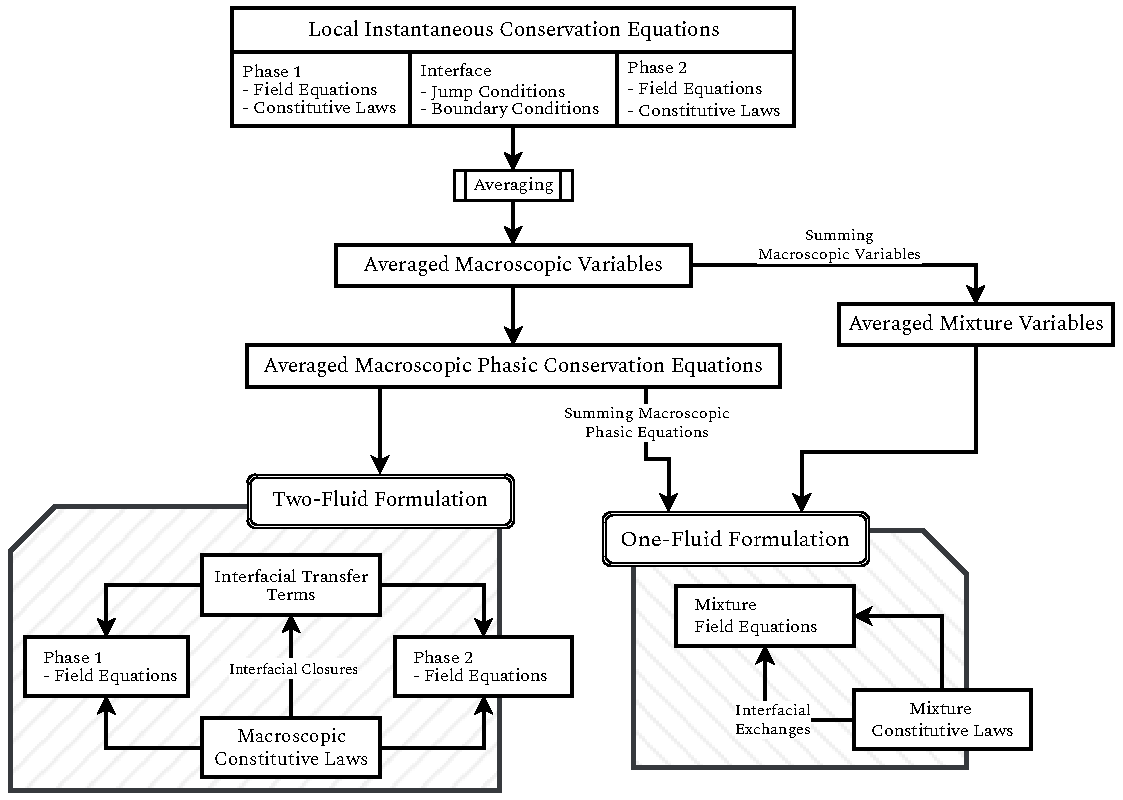
\includegraphics[width=1.\linewidth]{./Chapters/Chap1/figs/flowchart_multiphase2}
\caption{Two-phase flow formulations.}
%\label{\fig{rt_conv_3000}} % \fig used here
\end{figure}
\subsubsection{The One-Fluid Formulation}\label{sec:one-fluid}
In order to account for the varying material properties when representing
 two-phase flow as a single fluid, the mixture properties are defined in the 
 volume element \(V\). 
 The mixture density \(\rho\), viscosity \(\mu\), and thermal conductivity \(k\) 
 are defined as
\begin{subequations}
 \begin{align}
   \rho &\;=\;\textstyle\sum\nolimits_{\ind{i}} \alpha_{\ind{i}} \rho_{\ind{i}}\,,\\
   \mu &\;=\; \textstyle\sum\nolimits_{\ind{i}} \alpha_{\ind{i}} \mu_{\ind{i}}\,,\\
   k &\;=\; \textstyle\sum\nolimits_{\ind{i}} \alpha_{\ind{i}} k_{\ind{i}}\,.
 \end{align}
\end{subequations}
 Here, the properties \(\rho_{\ind{i}}\), \(\mu_{\ind{i}}\), and \(k_{\ind{i}}\) are phase intrinsic averages.
 Using the defined mixture density \(\rho\), the velocity, specific heat, and enthalpy can 
 be also defined as mass averaged mixture values.
\begin{subequations}\label{eq_vof_defs}
\begin{align}
  \vect{v} &\;=\; \textstyle\sum\nolimits_{\ind{i}} \alpha_{\ind{i}} \rho_{\ind{i}} \vect{v}_{\ind{i}}/ \rho,\\
  C_{p} &\;=\; \textstyle\sum\nolimits_{\ind{i}} \alpha_{\ind{i}} C_{p,\ind{i}} \rho_{\ind{i}}/\rho,\\
  H &\;=\; \textstyle\sum\nolimits_{\ind{i}} \alpha_{\ind{i}} \rho_{\ind{i}} \mathrm{H}_{\ind{i}}/\rho + |\vect{v}|^{2}/2\,,\text{where \(\vect{v}\) is the mixture velocity}. 
\end{align}
\end{subequations}

\subsubsection{The Two-Fluid Formulation}\label{sec:two-fluid}
Considering the volume element \(V\) as described in the previous section, 
 the volume fractions of the two phases \(\alpha_{\ind{i}}\,,\,i \in \{\ind{l},\ind{v}\}\) must satisfy the continuity constraint 
 \begin{equation}\label{eq:vol-frac-cont}
  \sum_{\ind{i}}\alpha_{\ind{i}}\;=\;1\,.
 \end{equation}
 The volume of the phase \(\ind{i}\) is given as 
 \begin{equation}
  V_{\ind{i}} = \integ{V}{} \alpha_{\ind{i}}\,\diff{V}\,.
 \end{equation}
 The ratio \(V_{\ind{i}}/V\) of the effective volume of the phase \(\ind{i}\) to the total volume is defined as 
 the void fraction of the phase. 
 
The averaged macroscopic equation for the conservation of mass is given in~\eq{eq:emp-mass}.
 The density and velocity of the phase \(\ind{i}\) is denoted by \(\rho_{\ind{i}}\) and \(\vect{v}_{\ind{i}}\).
 The interfacial mass transfer unit volume between the two phases is denoted
 by \(\Gamma\) and the surface area vector of the 
 volume element is denoted by \(\vect{a}\). With an additional phase mass source term \(\mathcal{S}_{\ind{i}}^{\alpha}\),
 the conservation of mass for a generic phase \(\ind{i}\) is 
 \begin{equation}\label{eq:emp-mass}
\pderiv{}{t}
\integ{V}{} \alpha_{\ind{i}} \rho_{\ind{i}} \,\diff{V}
+ \ointeg{\partial V}{} \alpha_{\ind{i}} \rho_{\ind{i}} \vect{v}_{\ind{i}} \cdot \diff{\vect{a}}\;=\;
\integ{V}{} \Gamma_{\ind{i}} \,\diff{V}
+ \integ{V}{} \mathrm{S}^{\alpha}_{\ind{i}} \,\diff{V}\,.
\end{equation}

The governing equation for the conservation of momentum is given in~\eq{eq:emp-mom}.
 The equation describes the change in momentum of the phase \(\ind{i}\) due to the effects of the
 fundamental forces in the system along with the effects of any internal forces or potentials \((\vect{F_{int}})_{\ind{i}}\)
 or any phase momentum source terms \(\vect{S}_{\ind{i}}^{\alpha}\). The pressure and gravitational acceleration are given as \(p\) and \(\vect{g}\) respectively.
 The stress tensor \(\tens{T}_{\ind{i}}\) comprises the molecular and turbulent stress tensors. Turbulence
 is addressed in~\sect{sec:turbs}.
\begin{equation}\label{eq:emp-mom}
\begin{split}
\pderiv{}{t}
\integ{V}{} \alpha_{\ind{i}} \rho_{\ind{i}} \vect{v}_{\ind{i}} \,\diff{V}
+ \ointeg{\partial V}{} \alpha_{\ind{i}} \rho_{\ind{i}} \vect{v}_{\ind{i}} \otimes \vect{v}_{\ind{i}} \cdot \diff{\vect{a}}
&\;=\; 
\integ{V}{} \left(-\alpha_{\ind{i}} \nabla p 
+ \alpha_{\ind{i}} \rho_{\ind{i}} \vect{g}
+ (\vect{F_{int}})_{\ind{i}} \right) \,\diff{V}
+ \ointeg{\partial V}{} \left[ \alpha_{\ind{i}} \left( \tens{T}_{\ind{i}}\right) \right] \cdot \,\diff{\vect{a}} \\
&\qquad {} + \integ{V}{} \vect{S}^{\alpha}_{\ind{i}} \,\diff{V}
+ \integ{V}{}  \bigl(\Gamma_{\ind{i}} \vect{v}_{\ind{i}} + \vect{\mathcal{M}}_{\ind{i}}\bigr)  \,\diff{V}\,.
\end{split}
\end{equation}

The momentum transfer term \(\vect{\mathcal{M}}_{\ind{i}}\) accounts for the momentum transfer from 
 the phase \(\ind{i}\) to the interface. This term also accounts for the momentum transfer
 due to interfacial mass transfer and is further detailed in~\sect{sec:closures}. It is only non-zero in case 
 of a relative motion between the phases and is subject to the constraint.

The averaged macroscopic formulation of the conservation of energy in the two-fluid formulation is 
 shown in~\eq{eq:emp-en}. The equation accounts for the change of the total energy \(E_{\ind{i}}\) in the 
 volume \(V\) due to the work done by line, surface, and volume (body) forces on the volume element,
 any heat transfer (in this specific case, only conduction and convection are considered),
 and due to the interfacial mass transfer in the volume element. 
 
\begin{align}\label{eq:emp-en}
\pderiv{}{t}
\integ{V}{} \alpha_{\ind{i}} \rho_{\ind{i}} E_{\ind{i}} \,\diff{V}
+ \ointeg{\partial V}{} \alpha_{\ind{i}} \rho_{\ind{i}} H_{\ind{i}}&
\vect{v}_{\ind{i}} \cdot \diff{\vect{a}}
\;=\;
\ointeg{\partial V}{} \alpha_{\ind{i}} (k_{\mathrm{eff}})_{\ind{i}} \nabla T_{\ind{i}} \cdot \diff{\vect{a}}
+ \ointeg{\partial V}{} \tens{T}_{\ind{i}} \vect{v}_{\ind{i}} \cdot \diff{\vect{a}}\nonumber \\
& + \integ{V}{} \vect{f_{b}}_{\ind{i}} \cdot \vect{v}_{\ind{i}} \,\diff{V}
+ \integ{V}{} \mathrm{S}_{u,\ind{i}} \,\diff{V} + \integ{V}{} \bigl(\Gamma_{\ind{i}}H_{\ind{i}} + \mathcal{E}_{\ind{i}}\bigr)\,\diff{V}\,.
\end{align} 

Having each transfer process of each phase balanced separately, 
 the two-fluid formulation is much more complex and requires closure models
 for each interaction. It is, simultaneously, a much more
 complete and general description of two-phase flow - accounting for the dynamic and non-equilibrium 
 interactions between the phases. The mixture or the two-fluid model do not retain information about the interface topology.
 Given a certain void fraction of a phase the two models are
 unable to comment on the nature of the flow regime.~\cite{ishiiThermoFluidDynamicsTwoPhase2011}


\subsection{Modelling Turbulence}\label{sec:turbs}
Flows are generally turbulent. Turbulence is characterised by irregular fluid motion dominated by
 eddies and vortices across a wide range of spatial and temporal scales. The largest eddies
 extract kinetic energy from the mean flow, which is then, through a cascade, transferred
 to the eddies at
 the smallest scale where the energy is dissipated due to viscosity, raising the 
 internal energy of the fluid~\cite{gilmanDevelopmentGeneralPurpose2014, davidsonIntroductionTurbulenceModels}.

RANS models result from decomposing flow variables into
 mean and fluctuating components, \(\displaystyle \phi = \overline{\phi} + \phi'\), applying Reynolds averaging,
 which filters out turbulent fluctuations below the
 averaging scale~\cite{besnardTurbulenceMultiphaseFlow1988a, hirschNumericalComputationInternal2007}.
 This operation yields additional Reynolds stress terms representing
 momentum transport by turbulence, which require closure.
 In order to draw closure relations, eddy-viscosity models of turbulence assume that:
 \begin{itemize}
    \item the turbulent scalar flux vector aligns with the mean scalar gradient.
    \item the Reynolds stress tensor is proportional to the mean velocity strain rate through an eddy viscosity.
 \end{itemize}
 While these assumptions simplify modelling, they tend to be, more often than not, invalid
 as they do not fully capture turbulence physics, especially in anisotropic 
 or non-equilibrium flow~\cite{popeTurbulentFlows2015}. This limitation can be significant
 in regions with complex strain rates or strong secondary flows.

Although turbulence can be modelled in various ways to various levels of resolutions,
 no general purpose turbulence model exists that accurately captures all flow scenarios.
 Turbulence in this study has been modelled using the Shear Stress Transport (SST) k-\(\omega\) model.
 The SST k-\(\omega\) model is a two-equation eddy-viscosity turbulence model
 based on the Reynolds-Averaged Navier-Stokes (RANS) equations.
 The model combines the advantages of the \(k\)-\(\omega\) model near walls - which
 accurately resolves boundary layer behaviour - and the \(k\)-\(\varepsilon\) model in
 the free stream, enhancing robustness and accuracy in separated flows~\cite{wilcoxTurbulenceModelingCFD2006}.
 The SST approach uses a blending function to smoothly transition between these models,
 which is especially effective in flows with strong adverse pressure gradients and separation,
 such as multiphase cavity flows~\cite{Menter1994}. Another blending function limits the eddy viscosity 
 in wake regions and a cross-diffusion term ensures consistency between the \(k\)-\(\omega\) and \(k\)-\(\varepsilon\)
 models.

The SST k-\(\omega\) models the eddy-viscosity \(\mu_{t}\) as
\begin{equation}
  \mu_{t}\;=\;\rho k T_{t}\,,
\end{equation}
 where \(T_{t}\) is the turbulent time scale defined using the k-\(\omega\) parameter \(\beta^{*}\) and the dissipation rate.
 The turbulent time and scales, along with the Kolmogorov time and length scales, and the Taylor microscale are defined below.
 \begin{subequations}
  \begin{align}
    T_{t}&\;=\; \bigl(\beta^{*}\,\omega\bigr)^{-1}\,,\\
    l_{t} & \quad \text{(definition omitted here)}
  \end{align}
\end{subequations}
Since the form of the RANS governing equations remains similar to the governing equations described in the
 previous section, they are not explicitly written here but can be found in the Star-CCM+ documentation~\citelater{starccm}.
 The additional equations accounting for the transport of the turbulent kinetic energy and dissipation rate 
 is given in~\eqref{eq:turbs-kw}
 \begin{subequations}\label{eq:turbs-kw}
\begin{align}
    \pderiv{}{t} \rho k  + \nabla \cdot (\rho k \vect{\overline{v}}) &= \nabla \cdot \left[(\mu + \sigma_{k} \mu_{t}) \nabla k\right] + P_k
        - \rho \beta^{*} f_{\beta^{*}} (\omega k - \omega_0 k_0) + S_k,\\
    \pderiv{}{t} \rho \omega + \nabla \cdot (\rho \omega \vect{\overline{v}}) & = \nabla \cdot \left[(\mu + \sigma_{\omega} \mu_t) \nabla \omega\right] + P_{\omega}
        - \rho \beta f_{\beta}(\omega^{2} - \omega_{0}^{2}) + S_{\omega},
\end{align} 
 \end{subequations}
 The turbulent viscosity, \(\mu_t\), is calculated as \(\mu_{t} = \rho k T_{t}\), where \(T_{t}\) is the turbulent time scale. 
 where \(\sigma_{k}\) and \(\sigma_{\omega}\) are the Prandtl numbers for \(k\) and \(\omega\) respectively.

\subsection{Modelling Vaporisation}
\subsection{Modelling Subproblem 1}
Not considering the mixing effects that might occur at later times, the infiltrating
 water into the evaporation chamber is a separated flow problem due to the sharp interface
 separating the two phases - water and air.
 
The objective - we want to understand the development of the flow field, 
 understand the amount of sloshing that can be expected in the system, and the amount of
 mixing that happens during the injection process and what the result flow system might look like 
 before the evaporation step. 

%The fundamental forces active in the system are the inertial, gravitational, viscous,
% pressure, and surface tension forces. The governing equations are analogous to the 
% governing equations of the homogenous two-fluid flow model.
% The flow field is described using the primary variables for each phase - $\rho_{i}, \vec{u}_{i}, E_{i}$.

\begin{itemize}
   \item what we're looking for and why we're interested in this
   \item phases involved, forces active and stuff
   \item assumptions we make
   \item variables we care about
   \item governing eqs (?)
   \item 3D vs 2D
\end{itemize}

\subsection{Modelling Subproblem 2}
\begin{itemize}
  \item from the top 
\end{itemize}